\part{Counting Solutions by Tensor Contraction}\label{part:count}

This chapter presents methods to count via tensor contractions. Starting first with Boolean tensor contractions, the chapter ends with tensor contractions for edge coloring's of 3-regular planner graphs.  The chapter follows partially \cite{2015JSP...160.1389B} and less so \cite{Penrose} as presented in \cite{biamonte2017tensor}. 

\section{Returning to Boolean Quantum States}

Boolean states were considered in detail in \S~\ref{sec:btn}, while properties of Boolean algebra are reviewed in Appendix \ref{sec:Boolean}.  Here we again recall certain key notations, 
with a succinct presentation tailored towards the use of tensor networks for counting \cite{2015JSP...160.1389B, VTN, Morton_2012, 2012PhRvL.109c0503C,Kourtis2019}.  

\begin{remark}
A quantum state is called {\it Boolean} if and only if it can be written in a local basis with amplitude coefficients taking only binary values $0$ or $1$. We relate such states with Boolean functions, allowing for a host of tools from algebra to be applied to their analysis. The present note derives several relations of these states, related to the contraction of the corresponding tensor networks.   
\end{remark}

\begin{remark}
 Note that {\it quantum Boolean functions} have alternatively been studied \cite{cj10-01} as unitary projectors (for unitary projector $f$,  spec($f$)$\in\{0,1\}$). 
\end{remark}

\begin{remark}[Notation]
We use $\7B$ to denote a Boolean bit, given by an element of the set $\{0,1\}$.  
A number in $\7B^n$ then denotes an $n$-long Boolean bit string.  If $x$ is a bit string, 
then we use $\ket{x}$ as an index for a basis state.  
If $f:\7B^n\rightarrow \7B$ then $\ket{f(x)}$ also indexes a basis state.  
\end{remark}

\begin{definition}[The class of Boolean quantum states \cite{2015JSP...160.1389B}]
 Let 
 \be 
 f:\7 B^n \rightarrow \7B
 \ee 
 be any switching function.  Then 
 \be 
 \psi_{\7 B} = \sum_{\x} \ket{\x}\ket{f(\x)}
 \ee 
 is an arbitrary representative in the class of Boolean states.  In this fashion, every Boolean function gives rise to a quantum state.  Conversely, every quantum state written in a local basis with amplitude coefficients taking binary values in $\{0,1\}$ gives rise to a Boolean function.  This defines the so called, class of Boolean quantum states \cite{CTNS}.
\end{definition}

\begin{theorem}[Boolean tensor network states \cite{CTNS}]\label{theorem:btns}
 A tensor network representing a Boolean quantum state is determined from the classical network description of the corresponding function.  
\end{theorem}

Theorem \ref{theorem:btns} was developed in \S~\ref{sec:btn}, where the quantum tensor networks are found by letting each classical gate act on a linear space and from changing the composition of functions, to the contraction of tensors.  


\subsection*{Contracting networks to solve SAT instances} 

\begin{theorem}[Counting 3-SAT solutions]\label{theorem:3-SAT}
Let $f$ be given to represent a 3-SAT instance. Then the standard two-norm length squared can be made to give the number of satisfying assignments of the instance \cite{2015JSP...160.1389B}.

\begin{proof}
 The quantum state takes the form 
 \be
 \psi_f = \sum_{\x} \ket{\x}\braket{f(\x)}{1} = \sum_{\x} f(\x) \ket{\x}
 \ee 
 We calculate the inner product of this state with itself viz 
 \be 
 ||\psi||^2=\sum_{\x \y} f(\x) f(\y) \langle \x, \y\rangle = \sum_\x f(\x) 
 \ee 
 which gives exactly the number of satisfying inputs.  This follows since $f(\x)f(\y)=\delta_{\x\y}$.   
 We note that for Boolean states, the square of the two-norm in fact equals the one-norm.  
\end{proof}
\end{theorem}



\begin{remark}[Counting 3-SAT solutions]
  We note that solving the counting problem \eqref{theorem:3-SAT} for general formula is known to be {\sf \#P}-complete.
\end{remark}


\begin{corollary}[Solving 3-SAT instances] 
 The condition 
 \be 
 ||\psi_f|| > 0
 \ee 
 implies that the SAT instance corresponding to $f$ has a satisfying assignment.  Determining if this condition holds for general Boolean states is 
 an {\sf NP}-complete decision problem.\sn{Instead of SAT, sometimes the term UNIQUE-SAT or USAT is used to describe the problem of determining whether a formula known to have either zero or one satisfying assignments has zero or has one.}  Note that determining this for 
 \be 
 \psi_{\overline f} = \sum_{\x} \ket{\x}\braket{f(\x)}{0} = \sum_{\x} (1-f(\x)) \ket{\x}
 \ee
 in general is a tautology problem.   
\end{corollary}

\subsection*{Graphical depiction and physicality} 

\begin{remark}[Graphical depiction]
 The algorithm is depicted below.  (a) gives a network realization of the function and determining if the network in (b) contracts to a value greater than zero solves a SAT instance.   
\begin{center}
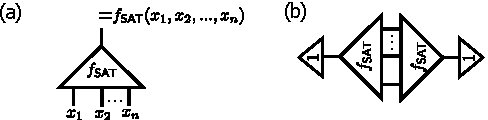
\includegraphics[width=10\xxxscale]{SAT1}
 %\epsfig{figure=SAT,width=10cm}
\end{center}
\end{remark}

As it happens, some time ago Penrose proved a theorem which applies directly to the physicality of Boolean satisfiable states.  
We changed the wording of the theorem only slightly, changing spin network to tensor network.  

\begin{theorem}[Penrose, 1967]
 The norm of a tensor network vanishes iff the physical situation it represents is forbidden by the rules of quantum mechanics \cite{Penrose67}. 
\end{theorem}

The above theorem applies to quantum states.  Consider instead a process that involved the impossibility of measuring a state to be in 
a certain state.  To capture when such a process is impossible, we modify Penrose's theorem as follows.  

\begin{corollary}[Forbidden process]
 The contraction of a tensor network vanishes iff the physical situation it represents is forbidden by the rules of quantum mechanics.  
\end{corollary}


\begin{example}[Examples of Penrose's theorem]
 Consider a Bell state $\Phi^+ = \ket{00}+\ket{11}$.  The amplitude of the first party measuring $\ket{0}$ followed by the second party measuring $\ket{1}$ is zero. This vanishing tensor network contraction is given by $\braket{01}{\Phi^+}$.  A second example is found by considering the norm of a state $\ket{\psi}$ formed by a network of connected tensors, by taking an inner product with a conjugated copy of itself $\braket{\psi}{\psi}$.  If this inner product vanishes, the network necessarily represents a non-physical quantum state, by Penrose's theorem. 
\end{example}

\begin{corollary}
All physical Boolean states are satisfiable.  
\end{corollary}


\begin{remark}[read-once]
A function $f$ is called \textit{read-once} iff it can be represented
as a Boolean expression using the operations conjunction, disjunction and negation, in
which every variable appears exactly once. We call such a factored expression a read-once
expression for $f$.  These correspond exactly to fan-out only circuits.  From this structure we conclude directly that  
\end{remark}

\begin{corollary}
All \textit{read-once} formula are satisfiable \cite{2015JSP...160.1389B}.  
\end{corollary}

\begin{remark}[Quantum read-once]
A quantum quantum state is called read-once if it can be represented by a tensor tree containing only isometries.   
\end{remark}

\begin{corollary}
All quantum \textit{read-once} formula are satisfiable, with the evaluation of k-point functions polynomial in the particle number.  
\end{corollary}


\section{Returning to Stabilizer Tensor Theory} 

In \S~\ref{sec:stabtt}, we talked in detail about the Clifford group and
stabilizer theory.  In fact, we proved the following theorem, which
connects the theory of stabilizer states to the theory tensor networks
which represent pseudo Boolean forms, which we have developed in our work,
and presented in this book.  

\begin{theorem}[Stabilizer states as pseudo Boolean forms]
Let 
\be 
f, g, k:\7B^n\rightarrow \7B
\ee 
then the quantum state 
\be 
\psi_{\7B} = \sum (-1)^{f(\1 x)}(i)^{g(\1 x)}k(\1 x)\ket{\1 x}
\ee 
is sufficient to express any stabilizer state.  
\end{theorem}

We will now take a step in the other direction.  That is, we wish to
understand what Boolean states are stabilizer states.  Here we will
consider the class of linear quantum states.  We consider the general
theory elsewhere.  

\begin{definition}[The class of linear quantum states]
 We define the linear class of quantum states as quantum states of the
form 
 \be 
 \psi_{\oplus L} = \sum c_0\oplus c_1x_1\oplus c_2x_2\oplus ...\oplus
c_nx_n \ket{x_1, x_2, ..., x_n}
 \ee
 where $\forall i, c_i = 0,1$ selects the linear function uniquely.  (As
we have mentioned, $c_0=1$ results technically in the affine class of
classical circuits, but we still define this full class as, the class of
linear quantum states.) 
\end{definition}

Note that the laws of the algebra enforce the strong constraint, $x\oplus
x = 0$ and $0\oplus y = y$.  So we find immediately that we need only
consider two fully entangled states in this class, as every other state
is found from a direct product of states of this form.  The first is 
\be 
 \psi_1 = \sum x_1\oplus x_2\oplus ...\oplus x_n
\ket{x_1, x_2, ..., x_n}
\ee 
and the second is given by 
\be 
 \psi_2 = \sum 1\oplus x_1\oplus x_2\oplus ...\oplus x_n
\ket{x_1, x_2, ..., x_n}
\ee 
The tensor network differs only by contraction with the constant
$\ket{1}$.  $\psi_1$ is shown in (a) and $\psi_2$ is shown in (b).  
\begin{center}
 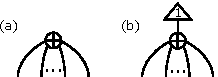
\includegraphics[width=0.45\textwidth]{linear-networks1} 
\end{center}

We will now consider the stabilizers of each of these cases, (a) and (b).  

\begin{remark}[Stabilizers of case (a)]
 The network in (a) is found from a Hadamard transform on all the legs of
a \COPY-tensor.  The $2^n$ stabilizers of the \COPY-tensor are generated
by the $n$ operators 
\be 
X_1\otimes X_2\otimes ...\otimes X_n
\ee 
\be 
Z_i\otimes Z_j, ~~~ 0 \leq i < j \leq n
\ee 
We have considered in lecture III how stabilizers transform.  Under the
Hadamard transform, the stabilizer generators transform to 
\be 
Z_1\otimes Z_2\otimes ...\otimes Z_n
\ee 
\be 
X_i\otimes X_j, ~~~ 0 \leq i < j \leq n
\ee 
\end{remark}


\section{Elementary Theorems of Tensor Contraction} 

The following can be used to prove graphical identities and represents a conceptual tool to aid 
in the analysis and design of tensor networks as a conceptual framework (as advocated in this lecture series) as well as a numerical tool for the simulation of quantum and classical physics.  

\begin{remark}[Linearity of tensor contraction] 
 Tensor contraction is linear in its arguments.  If $A$ is a tensor in a fully contracted network $\2C\{A\}$, if we let $A\mapsto A'+ B$ and then $A\mapsto kA$ we readily find that the contraction becomes $\2C\{A'\}+\2C\{B\}$ and $k\cdot \2C\{A\}$ respectively.  
\end{remark}


\begin{theorem}[Contraction to sum of products transform]
 Given a tensor $\Gamma^{...ijk}_{~~~~lmn...}$ in a fully contracted network (e.g.\ a network without open legs), the following graphical identity transforms the contraction, to a sum over products.  
\begin{center}
 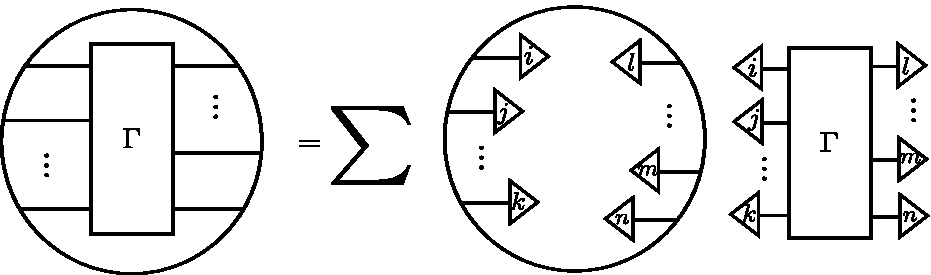
\includegraphics[width=0.65\textwidth]{contraction-2-+-over-prod} 
\end{center}
The circle is meant as an abstraction depicting a fully contracted but otherwise unknown network.  
\end{theorem}

\begin{theorem}[COPY-tensors as a resolution of identity]
The following sequence of graphical rewrites hold.  
\begin{center}
 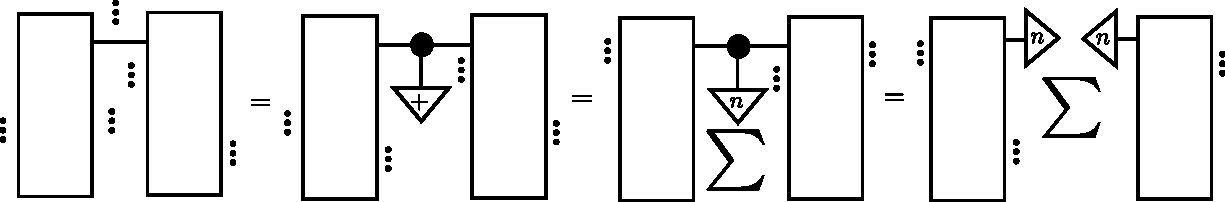
\includegraphics[width=0.95\textwidth]{wire-2-prod} 
\end{center}
\begin{proof}
In the above figure, on the left, we abstractly depict a other wise arbitrary tensor network, by showing only one single wire.  The unit for the COPY-tensor is the plus state $\ket{+}$.  This state is defined as a sum over basis states $\ket{n}$.  The tensor copies these basis states, and splits apart.  
\end{proof}
\end{theorem}





\begin{theorem}[A tensor contraction inequality]
Given a contracted network and a partition into two halves $x$, and $y$.  Writing the contraction as 
$\2C\{x,y\}$ the following inequality holds.  
\be 
\2C\{x,y\}\leq \2C\{x,x\}\cdot \2C\{y,y\}
\ee 
with graphical depiction.  
\begin{center}
 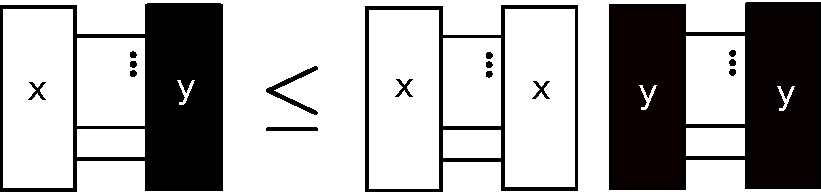
\includegraphics[width=0.67\textwidth]{tensor-ineq} 
\end{center}
\begin{proof}
 By the linearity of tensor contraction, we arrive at an abstract form of the 
 Cauchy-Schwarz inequality, with equality in the contraction iff $x = \alpha \cdot y$.  This leads 
 directly to the concept of an angle between tensors, 
 \be 
 \cos \theta_{xy} = \frac{\2C\{x,y\}}{\2C\{x\}\cdot \2C\{y\}}
 \ee
 where the right side is either real valued, or we take the modulus.  
\end{proof}
\end{theorem}







\section{A 3-fold way}  

We will now unify three concepts.  

\begin{remark}[Pseudo Boolean function]
 A function is called pseudo Boolean when it is total with type 
 \be 
 f(x): \7B^n \rightarrow \7C
 \ee 
\end{remark}





\subsection*{Fold I. Quantum States}

A quantum state is a map 
\be 
\psi: \7 C \rightarrow \2 H
\ee 
since $\psi (c) = c\cdot \psi\in \2 H$ for $c\in \7C$ and $\psi (1) = \psi$ uniquely determines $\psi$ by linearity.  We typically fix $\|\psi \|=1$.  Note that 
\be 
\braket{\psi}{i j\cdots k} = c_{i j\cdots k}
\ee 
where 
\be 
\psi = \sum_x c_x \ket{x}
\ee 
given basis $\ket{x}$.  We arrive at the following 
\be 
\exists ! f:\7B^n \rightarrow \7C ~|~ f(x)=c_x 
\ee 
and $f$ is pseudo Boolean and $\psi$ can be expressed as 
\be 
\psi = \sum_x f(x)\ket{x}
\ee 


\subsection*{Fold II. Linear Operators in $\2H\rightarrow \2H$} 

\begin{theorem}[Isomorphism between states and diagonal maps]
 There is an isomorphism sending every state $\psi\in \2 H$ to a diagonal map $\2 L(\psi) \in \2 H\rightarrow \2 H$.  Moreover, the eigenvalues of $\2 L(\psi)$ are the amplitudes of $\psi$ expressed in the spin basis. 
 \begin{proof}
 We write 
 \be
 \psi = \sum \alpha_\x \ket{\x}
 \ee 
 and then by constructing a map such that 
 \be 
 \ket{\x} \rightarrow \ket{\x}\ket{\x}
 \ee 
 one can construct $\2 L(\psi)$ as 
 \be 
 \2 L(\psi) =  \sum \alpha_\x \ket{\x}\bra{\x}
\ee
We then let 
\be 
\ket{+} := \ket{0} + \ket{1}+\cdots + \ket{n} 
\ee 
Assume we are considering $n$ qubits, then 
\be
\psi = 
 \2 L(\psi)\ket{+}^{\otimes n} 
 \ee 
 establishes the bijection.  We also note that 
 \be 
 \2 L(\psi)\ket{\1k} = \alpha_{\1k} \ket{\1k}
 \ee 
 satisfying the eigenvalue condition and hence, proving the result.  
\end{proof}
\end{theorem}



\begin{lemma}[Tensor networks equating states and diagonal maps]
The maps relied on in the above theorem can be given in terms of tensor networks.  
$\2 L(\psi)$ is shown in (a).  This map is invertible as shown in (b).  

\begin{center}
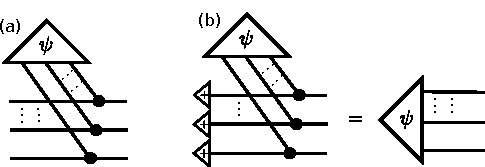
\includegraphics[width=12\xxxscale]{iso-states-diag-maps}
% 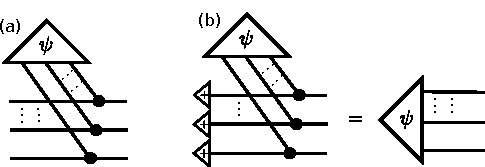
\epsfig{figure=iso-states-diag-maps,width=12cm}
\end{center}
\end{lemma}

\begin{remark}[Proof strategy]
Here we sketch what we call the argument by linearity.  We contract all wires of an open diagram as follows.  On the left we contract with $\bra{x,y,z}$ and on the right with $\ket{q,p,r}$.  
 \begin{center}
 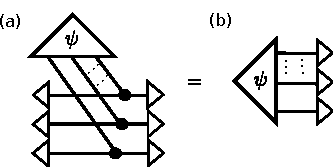
\includegraphics[width=8\xxxscale]{iso-states-diag-maps-proof}
% 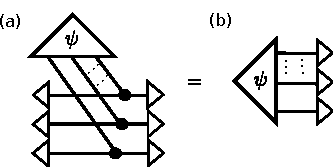
\epsfig{figure=iso-states-diag-maps-proof,width=8cm}
\end{center}
This is equivalent to evaluating the coefficients of three party delta functions as 
\be 
\delta_{xq}^{~~i}\delta_{yp}^{~~j}\delta_{zr}^{~~k}\psi_{ijk} = c_{ijk} ~ (=c_{xyz}=c_{qpr})
\ee 
by linearity, we recover the map $\2L(\psi)$. 
\end{remark}


\begin{remark}
 Note that from $\psi = \sum f(x) \ket{x}$ we have 
 \be 
 \2L (\psi) = \2 L \left( \sum f(x) \ket{x}\right) = \sum f(x) \2L (\ket{x}) = \sum f(x) \ket{x}\bra{x} 
 \ee 
\end{remark}


\subsection*{Fold III.  Classical Spin Hamiltonians} 
We will consider a generalized Ising spin Hamiltonian.  Let 
\be 
h = \sum h^i Z_i + \sum J^{ij}Z_i Z_j + \cdots + \sum k^{ij...k}Z_i Z_j \cdots Z_k 
\ee 
and let $s_i$ be a spin variable taking values $\pm 1$ and let $x_i$ be a Boolean valued $0,1$.  
Use 
\be 
s_i = 1 - 2 x_i 
\ee 
then 
\be 
Z_i = \I - 2 \ket{1}\bra{1}
\ee 
and so we arrive at 
\begin{equation} %\label{eq1}
\begin{split}
h_x & = \sum h^i (1 - 2 x_i) + \sum J^{ij}(1 - 2 x_i)(1 - 2 x_j) + \cdots \\  
 &~~~ + \sum k^{ij...k}(1 - 2 x_i) (1 - 2 x_j) \cdots (1 - 2 x_k) 
\end{split}
\end{equation}
and we arrive at the expression for $\psi$ 
\be 
\psi = \sum h_x(x) \ket{x} 
\ee 

In \cite{JDB08} we developed general methods to reason about spin Hamiltonians.  We explored an embedding reducing k-body interactions (e.g.\ $k^{ij...k}Z_i Z_j \cdots Z_k$) into two-body interactions by adding additional qubits.  

\subsection*{A three fold way}
We have shown that three different concepts, are effectively equivalent by constructing mathematical dualities that relate them precisely.  

\begin{center}
 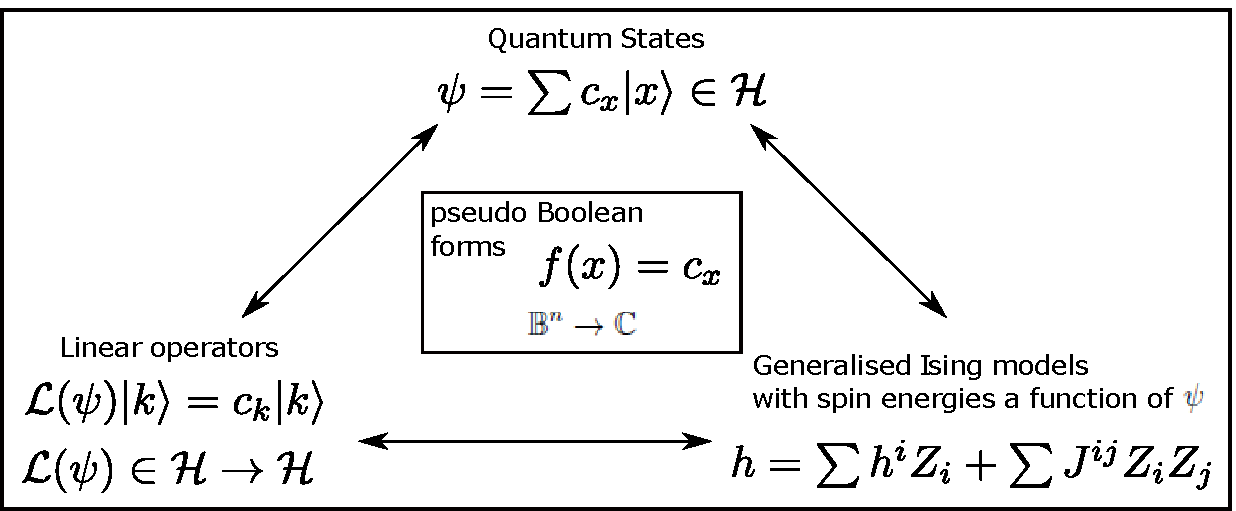
\includegraphics[width=0.95\textwidth]{3-fold-way} 
\end{center}


\begin{remark}[Factorization of quantum states into Tensor Networks]
 In the lectures, we also presented a universal a factorization of quantum states, into networks comprised of the building blocks (Quantum Legos), not included here. 
 A related factorization appeared in \cite{CTNS}.  
\end{remark}

\subsection*{Counting Graph Colorings}
Given a $3$-regular planar graph\sn{A graph is $k$-regular iff every node has exactly $k$~edges connected to it.},
how many possible edge colorings using three colors exist,
such that all edges connected to each node have distinct colors?
This counting problem can be solved in an interesting (if not computationally efficient) way
using the order-3 $\epsilon$~tensor, which is defined in terms of components as
\begin{align}
\notag
 &\epsilon_{012} = \epsilon_{120} = \epsilon_{201} = 1,\\
 &\epsilon_{021} = \epsilon_{210} = \epsilon_{102} = -1,
\end{align}
otherwise zero. The counting algorithm is stated as
\begin{theorem}[Planar graph $3$-colorings, Penrose 1971 \cite{Penrose}]\label{thm:3-color}
The number~$K$ of proper $3$-edge-colorings of a planar $3$-regular graph
is obtained by replacing each node with an order-3 epsilon tensor,
replacing each edge with a wire,
and then contracting the resulting tensor network.
\end{theorem}

We will first consider the simplest case, a graph with just two nodes.
In this case we obtain
\begin{center} 
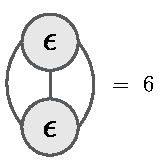
\includegraphics{epsilon-norm-6}
\end{center} 
There are indeed $6$ distinct edge colorings for this graph, given as
\begin{center}
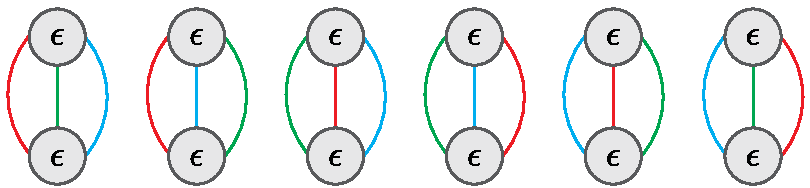
\includegraphics{color-norm} 
\end{center}
To understand Theorem~\ref{thm:3-color},
note first that the contraction~$K$ of the epsilon tensor network is the sum of all possible individual assignments of the index values
to the epsilon tensors comprising the network.
Each of the three possible index values can be understood as a color choice for the corresponding edge.
Whenever the index values for a given epsilon tensor are not all different, the corresponding term in~$K$ is zero.
Hence only allowed color assignments result in nonzero contributions to~$K$,
and for a graph that does not admit a proper $3$-edge-coloring we will have~$K=0$.
For instance, for the non-$3$-colorable Petersen graph we obtain
\begin{center}
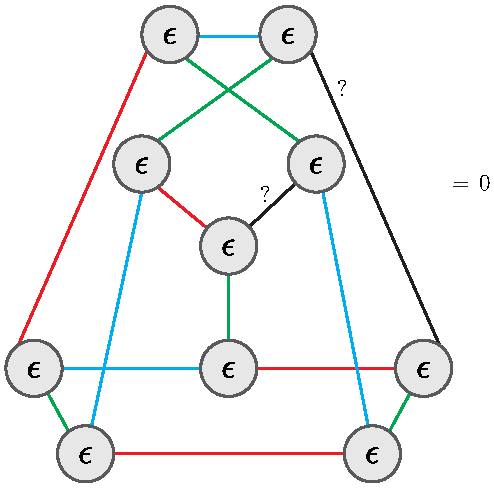
\includegraphics{petersen}
\end{center}

However, for~$K$ to actually equal the number of allowed colorings, each nonzero term must have the value~$1$ (and not~$-1$).
This is only guaranteed if the graph is planar,
as can be seen by considering the non-planar graph $K_{3,3}$:
\begin{center}
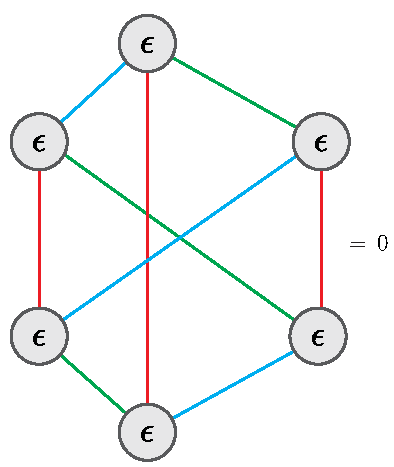
\includegraphics{k33}
\end{center}
The edges can be colored with three colors---in 12 different ways---yet the contraction vanishes.

The computational complexity of this problem has been studied in \cite{xia2007computational}. Interesting, by a well known result (Heawood 1897), the 3-colorings as stated above, are one quarter of the ways of coloring the faces of the graph with four colors, so that no 
 two like-colored faces have an edge in common. 
\begin{example}[Physical implementation of $\epsilon_{abc}$ in quantum computing]
In quantum computing, typically one works with qubits (two level quantum systems) but implementations using qutrits exist (three level quantum systems, available in e.g.~nitrogen vacancy centers in diamond---see for instance \cite{2014NatCo...5E3371D}). 
The epsilon tensor $\epsilon_{abc}$ could be realized directly as a locally invariant 3-party state using qutrits, and can also be embedded into a qubit system.  We leave it to the reader to show that by pairing qubits, $\epsilon_{abc}$ can be represented with six qubits, where each leg now represents a qubit pair.  (Note that a basis of 3 states can be isometrically embedded in 4-dimensional space in any number of ways.) Show further that the construction can be done such that the two qubit pairs (together representing one leg) are symmetric under exchange.
%Note the similarities with Eq.~\eqref{eqn:projaklt} in Example~\ref{ex:AKLT}.
\end{example}
 
\begin{myexercise}[Representation of the Epsilon Tensor on Qubit States]  
The epsilon tensor is typically considered 
 in $\7C^3\otimes \7C^3\otimes \7C^3$.  Show that by pairing qubits, this can be represented in the space $\7C^{2\otimes 6}$ of six qubits, where each leg now represents a qubit pair.  Show further that the construction can be done such that the two qubit pairs are symmetric under exchange. 
\end{myexercise}